\begin{prob}
    For a given graph $G$ with positive weights containing a node $v_0$, define $T_{\text{shortest}}(G, v_0)$ as the shortest path tree starting from $v_0$ (as given by Dijkstra's algorithm), and $T_{\text{MST}}(G, v_0)$ as the minimum spanning tree given by Prim's algorithm starting at $v_0$. 

    Find a small example graph $G$ \emph{with at most 4 nodes} where $T_{\text{shortest}}(G, v_0) \neq T_{\text{MST}}(G, v_0)$.
    \begin{soln}
        The idea is to notice that Prim selects the edge with the minimum weight from the current tree, while Dijkstra selects the node with the minimum distance from the inital node. 
        Thus we need to make it so that in the grpah, one edge is small enough that it will be selected by Prim, but will not be selected by Dijkstra because a "more direct" way exists.

        You can actually find one such graph with only 3 nodes. Here is a simple example:
    \begin{center}
        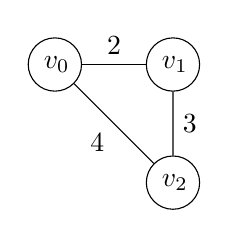
\begin{tikzpicture}[scale=1.5]
		    \tikzset{
   			vertex/.style={draw, circle, text width=8, align=center},
    		arc/.style={->}
		    }

   	        \draw node[vertex] (v0) at (0,0) {$v_0$};
            \draw node[vertex] (v1) at (1,0) {$v_1$};
            \draw node[vertex] (v2) at (1,-1) {$v_2$};
            % \foreach \x/\y in {%
        	%     s/a,s/c,c/a,a/b,b/c,b/d,d/c,b/t,d/t%
    	    % }{
   		 	% \draw (\x) edge[arc] (\y);
   	        % }
            \draw[] (v0) -- node[above] {2} (v1);
            \draw[] (v1) -- node[right] {3} (v2);
            \draw[] (v0) -- node[below left] {4} (v2);
	    \end{tikzpicture}
    \end{center}

    Prim will yield the following tree (total weight 5): 

    \begin{center}
        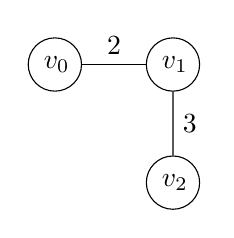
\begin{tikzpicture}[scale=1.5]
		    \tikzset{
   			vertex/.style={draw, circle, text width=8, align=center},
    		arc/.style={->}
		    }

   	        \draw node[vertex] (v0) at (0,0) {$v_0$};
            \draw node[vertex] (v1) at (1,0) {$v_1$};
            \draw node[vertex] (v2) at (1,-1) {$v_2$};
            % \foreach \x/\y in {%
        	%     s/a,s/c,c/a,a/b,b/c,b/d,d/c,b/t,d/t%
    	    % }{
   		 	% \draw (\x) edge[arc] (\y);
   	        % }
            \draw[] (v0) -- node[above] {2} (v1);
            \draw[] (v1) -- node[right] {3} (v2);
            % \draw[] (v0) -- node[below left] {4} (v2);
	    \end{tikzpicture}
    \end{center}

    But Dijkstra will yield the following tree (since the distance from $v_0$ to $v_2$ is 4 and not 5): 

    \begin{center}
        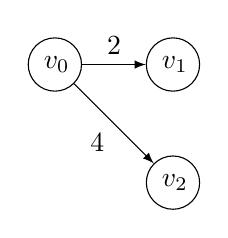
\begin{tikzpicture}[scale=1.5]
		    \tikzset{
   			vertex/.style={draw, circle, text width=8, align=center},
    		arc/.style={->}
		    }

   	        \draw node[vertex] (v0) at (0,0) {$v_0$};
            \draw node[vertex] (v1) at (1,0) {$v_1$};
            \draw node[vertex] (v2) at (1,-1) {$v_2$};
            % \foreach \x/\y in {%
        	%     s/a,s/c,c/a,a/b,b/c,b/d,d/c,b/t,d/t%
    	    % }{
   		 	% \draw (\x) edge[arc] (\y);
   	        % }
            \draw[-latex] (v0) -- node[above] {2} (v1);
            % \draw[] (v1) -- node[right] {3} (v2);
            \draw[-latex] (v0) -- node[below left] {4} (v2);
	    \end{tikzpicture}
    \end{center}

    \end{soln}
\end{prob}
